\documentclass[9pt]{beamer}
\usetheme{Warsaw}
\usepackage[utf8]{inputenc}
\usepackage[english]{babel}
\usepackage{amsmath}
\usepackage{amsfonts}
\usepackage{amssymb}
\usepackage{graphicx}
\usepackage{fontspec}
\newfontfamily\cjkfont{Noto Sans CJK SC} % Or any appropriate font you have
\author{leviathan/talamon\\(Lanceville Technology)}
\title{Breaking the microchip monopoly}
\setbeamercovered{transparent} 
\setbeamertemplate{navigation symbols}{} 
\logo{lsa.png} 
%\institute{} 
%\date{} 
\subject{A free semiconductor manufacturing standard}
\begin{document}

\begin{frame}
	\titlepage
	\begin{center}
		
\includegraphics[width=50pt,height=50pt]{lsa.png}
		\\ Libre Silicon Alliance
	\end{center}
\end{frame}

%\begin{frame}
%\tableofcontents
%\end{frame}

\section[What]{}
\begin{frame}{What we do}
	\begin{itemize}
        \setlength\itemsep{1em}
		\item We make \textbf{free silicon}
		\item Breaking the monopoly of big semiconductor manufacturers
		\item Eliminating the vendor lock-in to big semiconductor manufacturers
		\item Making semiconductor development super quick and inexpensive
		\item Introducing the LSPL (LibreSilicon public license)
		\item Attracting commercial design houses to develop \textbf{free silicon}
	\end{itemize}
\end{frame}

\section[Why]{}
\begin{frame}{Why are we doing this?}
	\begin{itemize}
		\item MPWs cost around 20'000 USD nowadays
		\item MPWs take around 2-9 months nowadays
		\item All manufacturers want NDAs (some NDAs even have NDAs!)
		\item Your design for a vendor process contains process specific design quirks (also under NDA!)
		\item No manufacturer provides the GDS2 files in order to manufacture the designs in your basement (there is \textbf{no} free silicon yet)
		\item You can't even publish your own designs!
	\end{itemize}
\end{frame}

\begin{frame}{Closed silicon market}
	\begin{center}
		\hspace*{-0.3in}
		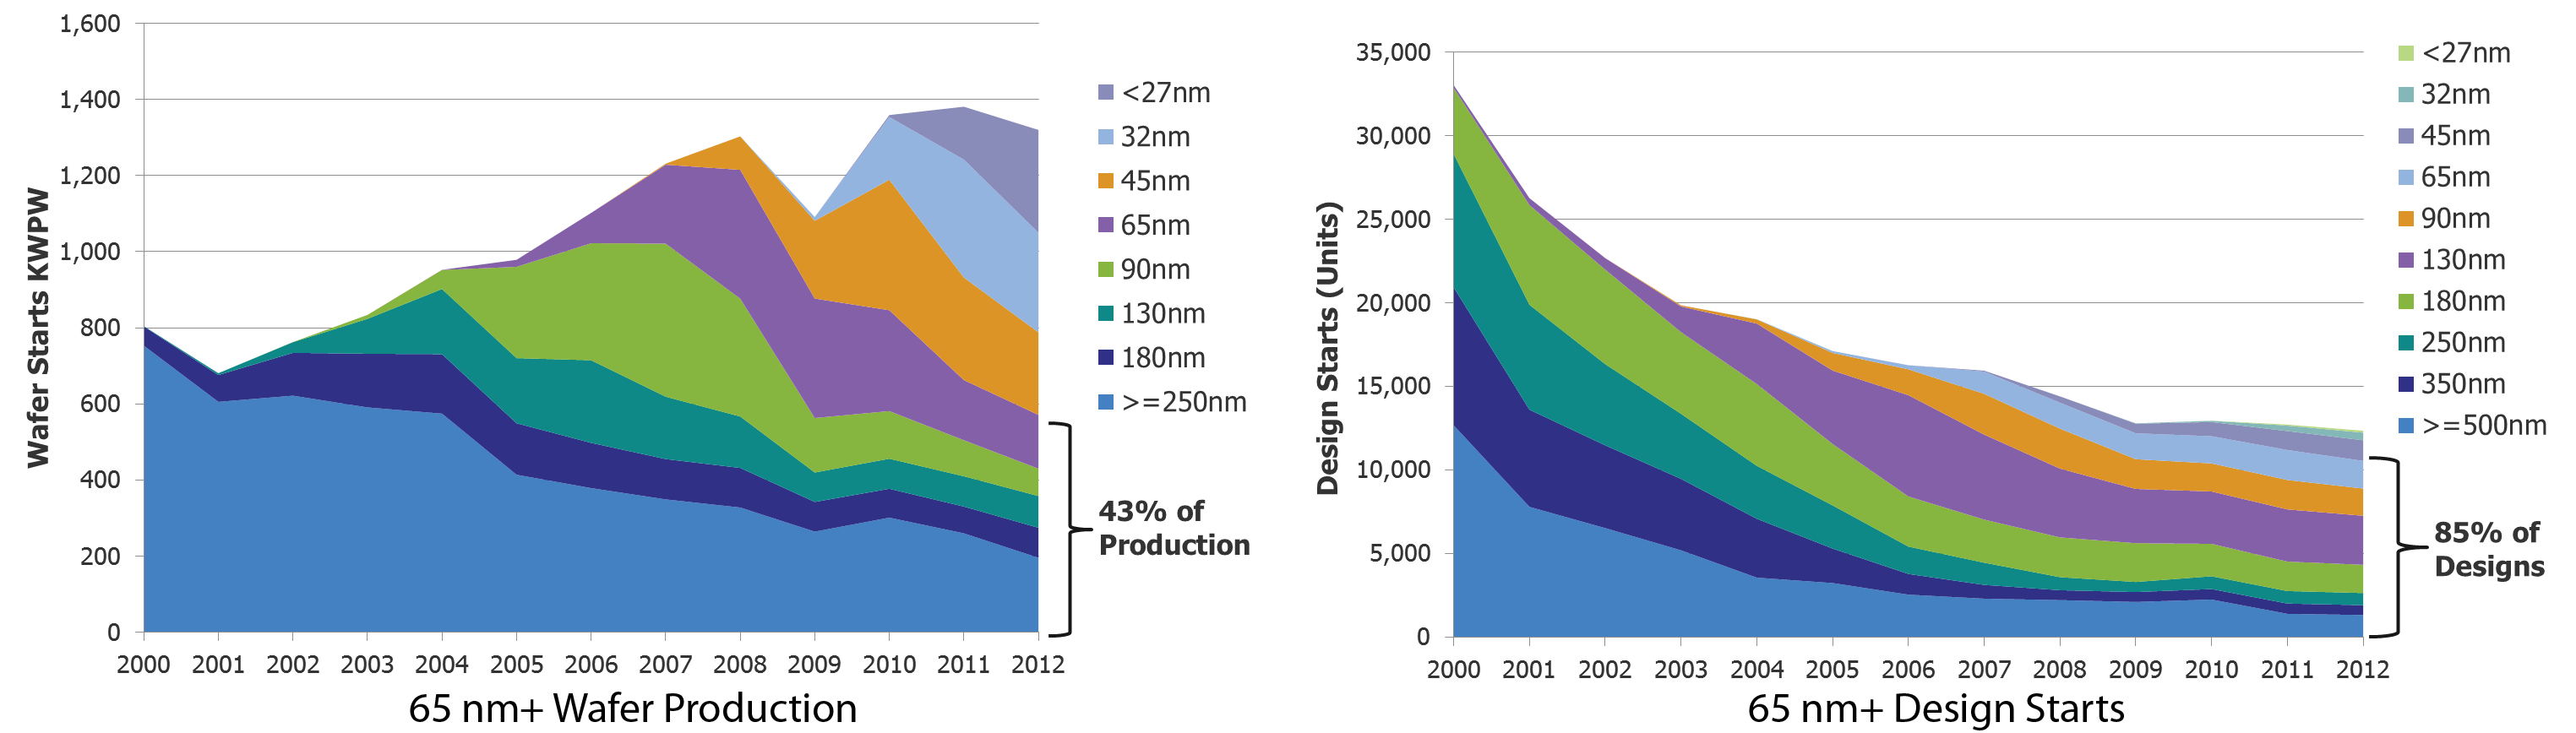
\includegraphics[width=1.15\textwidth]{market-closing.png} \\
	\end{center}
	
	\footnotetext[1]{http://semimd.com/favre/2016/08/24}
\end{frame}

\section[Who]{}
\begin{frame}{Community projects}
	\begin{center}
		
\includegraphics[width=100pt]{Icarus.png} \\
		
\includegraphics[width=100pt]{Yosys.png} \\
		
\includegraphics[height=50pt]{Opencircuit.png}
	\end{center}
\end{frame}

\begin{frame}{Companies and institutions}
	\begin{center}
		
\includegraphics[width=100pt]{HKUST_Logo.png}
		
\includegraphics[width=100pt]{NFF.jpg}  \\
		
\includegraphics[width=100pt]{efabless_logo.png} \\
		
\includegraphics[width=100pt]{Lanceville.png}
	\end{center}
\end{frame}

\section[How]{}
\begin{frame}{Reward IP developers}
	\begin{itemize}
        \setlength\itemsep{1em}
		\item Chip designer is rewarded when IP is used on collaboration platforms
		\item Smart contracts track usage and pay contributors
		\item Hash of IP + desired return value
	\end{itemize}
\end{frame}

\begin{frame}{How we do it}
	\begin{itemize}
		\item Introducing an open source chip manufacturing process standard specification
		\item Introducing a fully integrated free EDA for ASIC design\footnotemark
		\item Renting the clean room and manufacturing equipment at HKUST every 2 weeks for around 12 hours \\		
		\begin{center}
			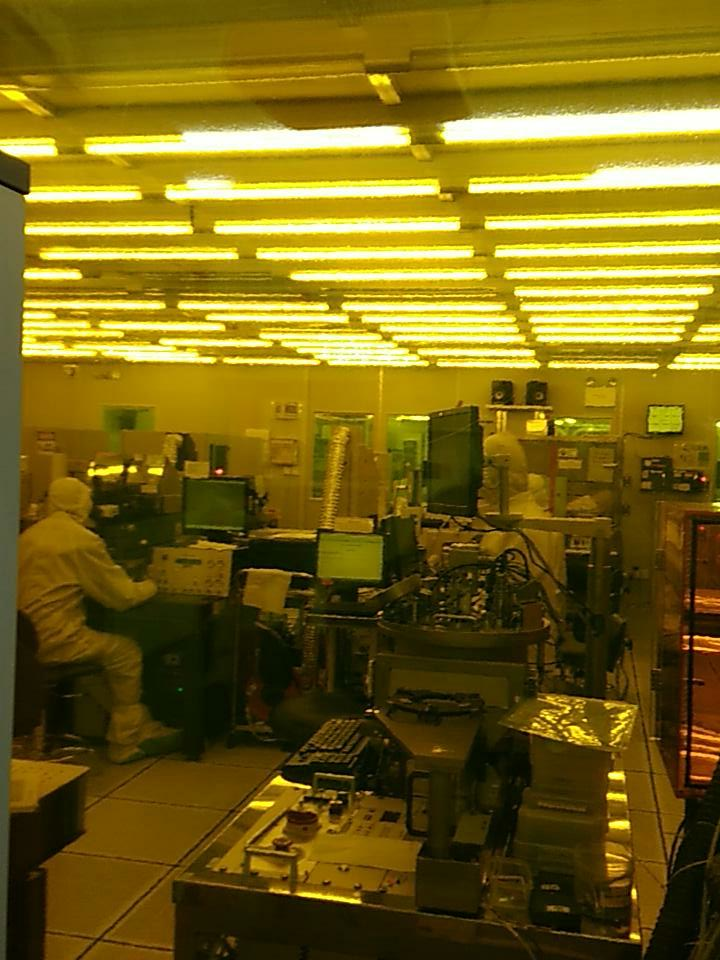
\includegraphics[height=100pt]{cleanroom.png}
			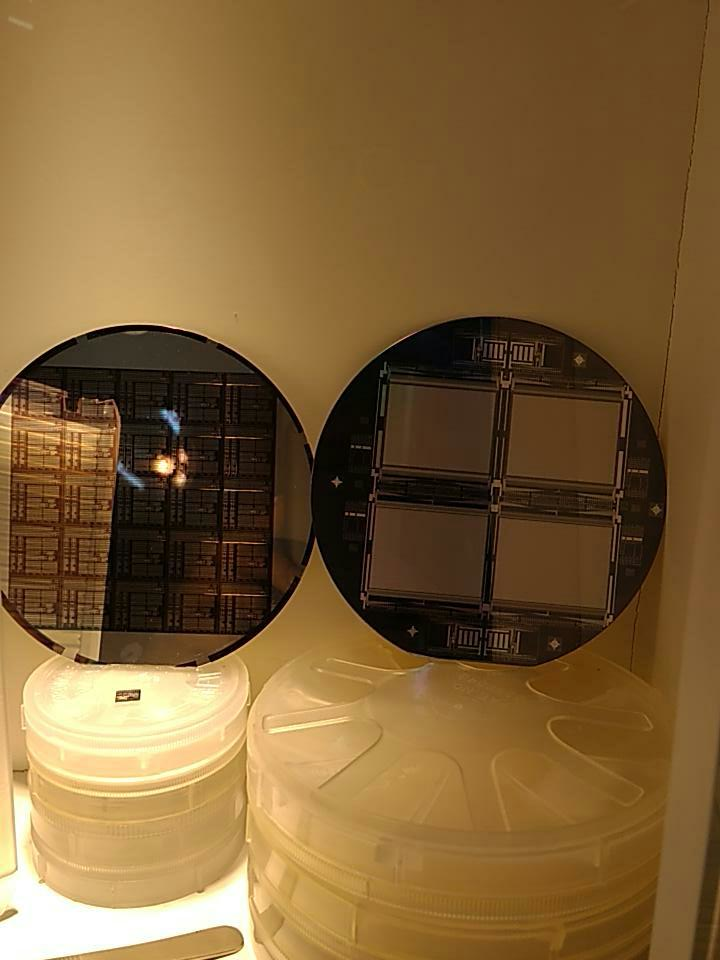
\includegraphics[height=100pt]{examples.png}
		\end{center}
	\end{itemize}

	\footnotetext[1]{https://github.com/leviathanch/qtflow}
\end{frame}

\begin{frame}{Libre Silicon EDA Tools}
	\begin{itemize}
		\item QtFlow EDA\footnotemark
		\begin{itemize}
				\item EDA suite written in Qt5
				\item Wave viewer
				\item Planned:
				\begin{itemize}
					\item Integration of higher level HDLs (CLash)
					\item Plugins through PythonQt
				\end{itemize}
		\end{itemize}
		\item Icarus Verilog simulation\footnotemark
		\item QRouter maze router\footnotemark
		\item GrayWolf floor planner\footnotemark
	\end{itemize}

	\footnotetext[2]{https://github.com/leviathanch/qtflow}
	\footnotetext[3]{http://iverilog.icarus.com}
	\footnotetext[4]{https://github.com/leviathanch/qrouter}
	\footnotetext[5]{https://github.com/leviathanch/graywolf}
\end{frame}

\begin{frame}{QtFlow screen shots}
	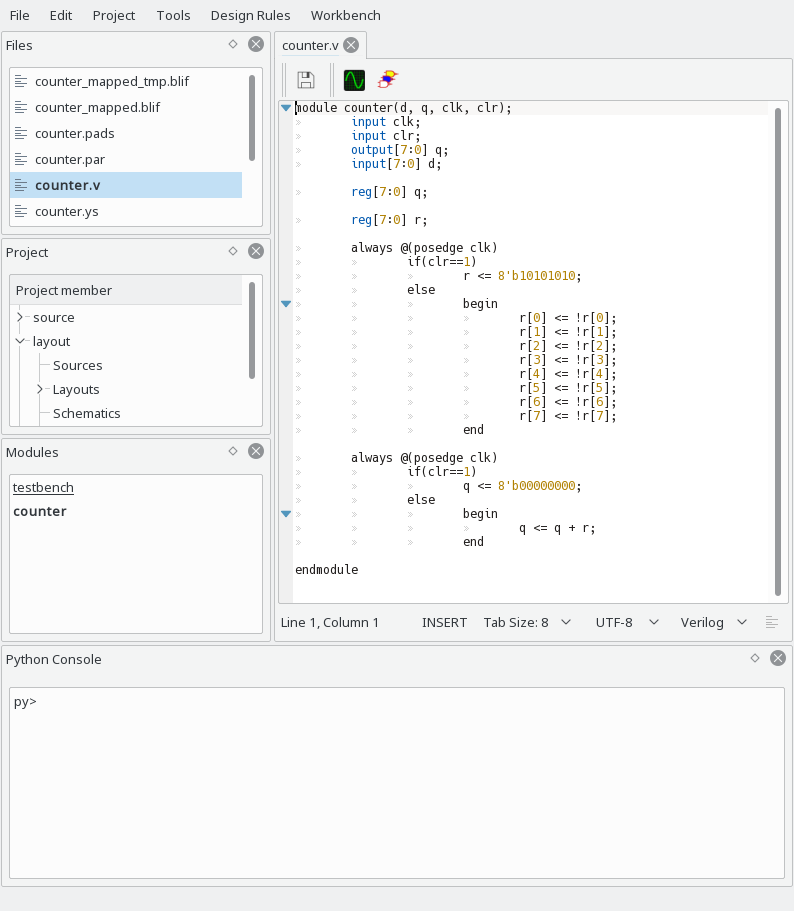
\includegraphics[width=100pt]{Screenshot_20171218_044022.png}
	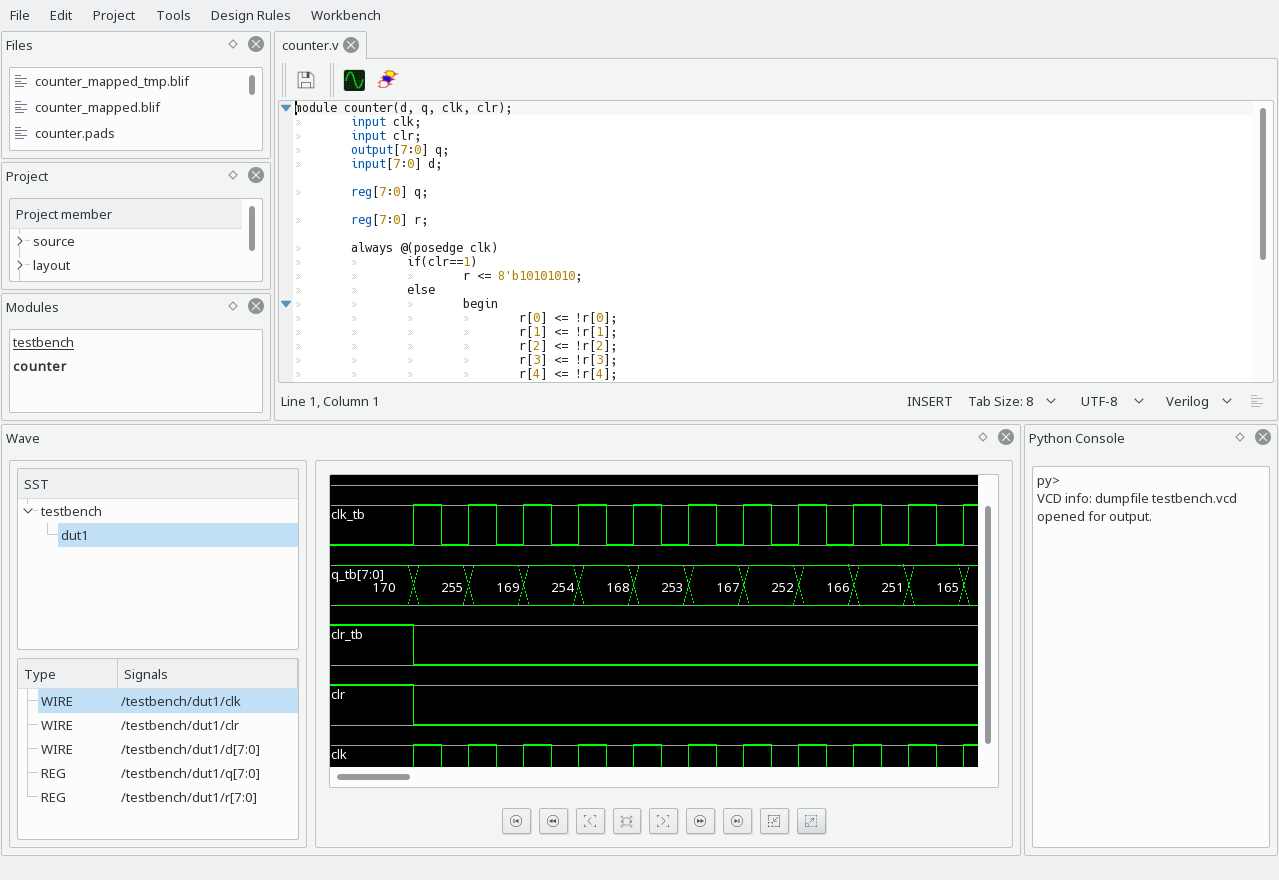
\includegraphics[width=100pt]{Screenshot_20171218_045118.png}
	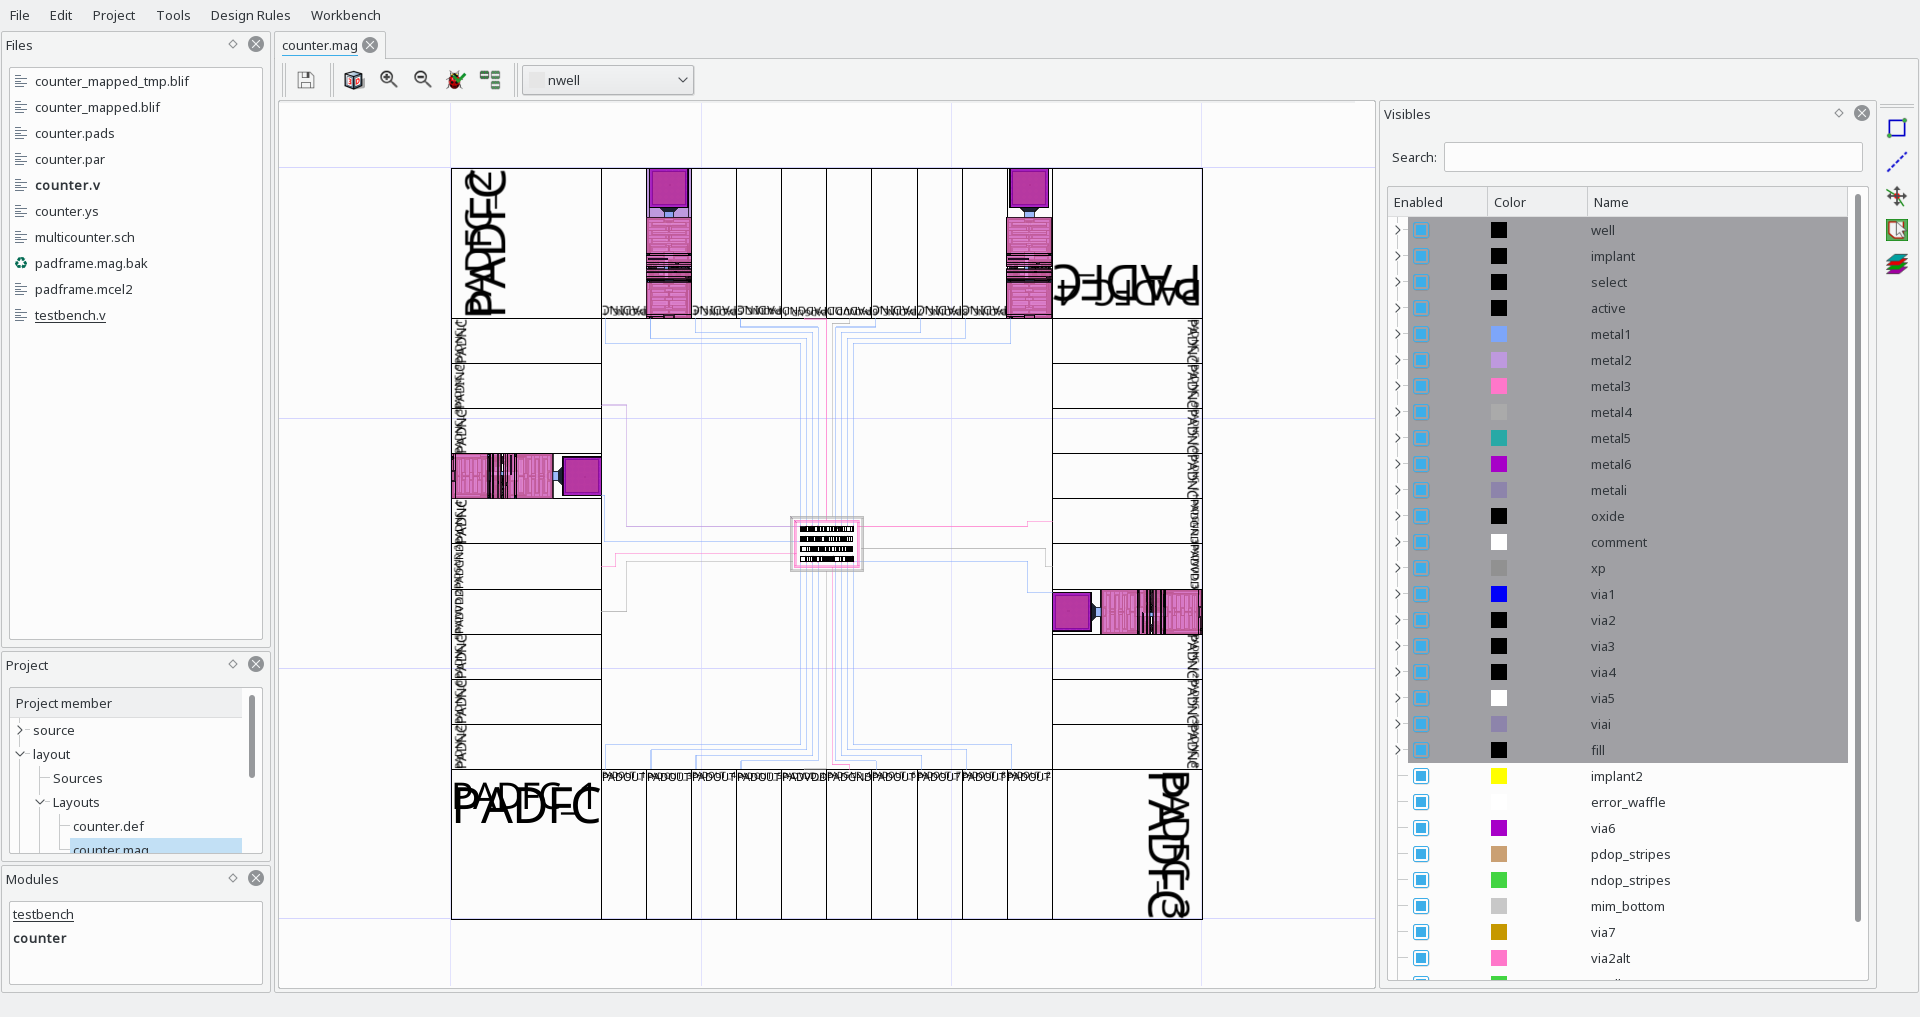
\includegraphics[width=100pt]{Screenshot_20171218_045416.png}
\end{frame}

\section[Conclusion]{}

\begin{frame}{Help needed}
	\begin{itemize}
		\item Work on developing QtFlow
		\begin{itemize}
			\item GrayWolf issues\footnotemark
			\item QRouter issues\footnotemark
			\item Front end issues\footnotemark
		\end{itemize}
		\item Work on the LibreSilicon process\footnotemark and technologies\footnotemark
		\begin{itemize}
			\item Work on the standard logic cells
			\item Work on developing FreeFLASH
			\item Work on developing FreeDRAM
			\item Develop ADCs and stuff
		\end{itemize}
		\item Financial contributions/Investments
	\end{itemize}

	\footnotetext[6]{https://github.com/leviathanch/graywolf}
	\footnotetext[7]{https://github.com/leviathanch/qrouter}
	\footnotetext[8]{https://github.com/leviathanch/qtflow}
	\footnotetext[9]{https://github.com/leviathanch/libresiliconprocess}
	\footnotetext[10]{https://github.com/leviathanch/ls018}
\end{frame}

\begin{frame}{Contact}
	\begin{block}{leviathan}
		Full name: David Lanzendörfer \\
		E-Mail (please use GnuPG if possible): david.lanzendoerfer@lanceville.cn \\
		Riot ID: @leviathanch:matrix.org \\
		Phone/NSA Chat(WhatsApp): +852 6672 2499		
	\end{block}
	\begin{block}{talamon}
		Full name: Andreas Westerwick \\
		E-Mail (please use GnuPG if possible): andreas.westerwick@o2s.ch \\
		Mumble: murmur.lanceville.hk
	\end{block}
\end{frame}

\begin{frame}{Thank you!}
	\begin{center}
		\textbf{Thank you very much!} \\
		\textbf{Vielen herzlichen Dank!} \\
		\textbf{\cjkfont 非常感谢你们!} \\
		
\includegraphics[width=100pt]{cat.png}
	\end{center}
\end{frame}

\end{document}
